\documentclass[
12pt, % 字体大小
a4paper, 
oneside, % 单面打印(双面为twoside)
headinclude,footinclude, % 页眉页脚包含在文本区域内,确保不被裁剪或掩盖
]{scrartcl}
% 主题和样式
\usepackage[
nochapters, % 无章节层级 
beramono, % 等宽字体样式
eulermath, % 数学公式Euler字体
pdfspacing, % 字间距
dottedtoc % 点线式目录
]{classicthesis}
\usepackage{arsclassica} 
%----------------------------------------------------------------------------------------
% 输入和页面排版
\usepackage[T1]{fontenc} % 字体编码
\usepackage[utf8]{inputenc} % 输入编码
\usepackage{ctex} % 汉语
\usepackage{amsmath,amssymb,amsthm} % 数学公式
\usepackage{indentfirst} % 缩进
\setlength{\parindent}{2em} % 段落缩进
\usepackage[
top=2cm,
bottom=2cm, 
left=2cm,
right=2cm, 
headheight=20pt, 
includeheadfoot 
]{geometry} % 页面
\usepackage{scrlayer-scrpage} % 页眉页脚
\renewcommand{\sectionmark}[1]{\markright{\spacedlowsmallcaps{#1}}}
\renewcommand{\subsectionmark}[1]{\markright{\thesubsection~#1}}
\lehead{\mbox{\llap{\small\thepage\kern1em\color{halfgray} \vline}\color{halfgray}\hspace{0.5em}\rightmark\hfil}} % 标题旁边标记页码
\cfoot{\hyperlink{toc}{\color{RoyalBlue}返回目录}} % 页脚返回目录链接
\pagestyle{scrheadings}
%----------------------------------------------------------------------------------------
% 图表和引用
\usepackage{graphicx} % 图像
\graphicspath{{Figures/}} % 图像路径
\usepackage{subfig} % 图组
\usepackage{float} % 浮动
\usepackage{enumitem} % 列表
\usepackage{varioref} % 交叉引用
%----------------------------------------------------------------------------------------
% 代码
\usepackage{listings}
\lstset{
    language=Matlab,
    basicstyle=\ttfamily\small,   % 字体
    numbers=left,                 % 行号
    numberstyle=\tiny\color{gray},
    stepnumber=5,
    numbersep=5pt,
    backgroundcolor=\color{white},% 背景
    tabsize=2,                    % 制表符宽度
    frame=single,                 % 边框
    captionpos=t,                 % 标题
    title=\lstname,
    breaklines=true,              % 换行
    breakatwhitespace=true,
    escapeinside={`}{`},          % 转义(中文注释)
}
\lstset{
    language=Python,            
    basicstyle=\ttfamily\small,   % 字体
    numbers=left,                 % 行号
    numberstyle=\tiny\color{gray}, 
    stepnumber=5,             
    numbersep=5pt,            
    backgroundcolor=\color{white},% 背景
    tabsize=4,                    % 制表符宽度            
    frame=single,                 % 边框
    captionpos=t,                 % 标题
    title=\lstname, 
    breaklines=true,              % 换行
    breakatwhitespace=false,   
    escapeinside={`}{`},          % 转义(中文注释)
}
\usepackage{algorithm} % 算法
\usepackage{algpseudocode}
\usepackage{mdframed} % 跨页框架
% 不浮动算法环境
\newcounter{myalgorithm}
\renewcommand{\themyalgorithm}{\arabic{myalgorithm}}
\newenvironment{myalgorithm}[1][]{
  \refstepcounter{myalgorithm}
  \begin{mdframed}[
    skipabove=\topskip,
    skipbelow=\topskip,
    needspace=3\baselineskip,
    linewidth=0.4pt,
    frametitlefont=\normalfont\bfseries,
    frametitle={算法 \themyalgorithm\if\relax\detokenize{#1}\relax\else:#1\fi},
    frametitlerule=true,
    frametitlerulewidth=0.4pt,
    repeatframetitle=true
  ]
  \begin{algorithmic}[1]
  \ifx\relax\detokenize{#1}\relax
    \addcontentsline{alg}{algorithms}{\makebox[7em][l]{算法~\themyalgorithm} }
  \else
    \addcontentsline{alg}{algorithms}{\makebox[7em][l]{算法~\themyalgorithm} #1}
  \fi
}{
  \end{algorithmic}
  \end{mdframed}
}
% 关键词
\algrenewcommand{\algorithmicwhile}{当}
\algrenewcommand{\algorithmicdo}{执行}
\algrenewcommand{\algorithmicend}{结束}
\algrenewcommand{\algorithmicif}{如果}
\algrenewcommand{\algorithmicthen}{那么}
\algrenewcommand{\algorithmicelse}{否则}
\algrenewcommand{\algorithmicfor}{对于}
\algrenewcommand{\algorithmicrepeat}{循环}
\algrenewcommand{\algorithmicuntil}{直到}
\algrenewcommand{\algorithmicloop}{循环}
\algnotext{EndFor}
\algnotext{EndIf}
\algnotext{EndLoop}
\algnotext{EndWhile}
%----------------------------------------------------------------------------------------
% 超链接与PDF信息
\usepackage{hyperref} 
\hypersetup{
colorlinks=true, % 彩色
breaklinks=true, % 断行
urlcolor=webbrown, % URL棕色
linkcolor=RoyalBlue, % 内部链接蓝色
citecolor=webgreen, % 引用绿色
bookmarks=true, % 书签
bookmarksnumbered,
pdftitle={}, 
pdfauthor={},
pdfsubject={}, 
pdfkeywords={}, 
pdfcreator={pdfLaTeX}, 
pdfproducer={LaTeX with hyperref and ClassicThesis} 
}
%----------------------------------------------------------------------------------------
% 目录与标题
\usepackage{titlesec} 
\AtBeginDocument{
    \renewcommand{\contentsname}{目\hspace{1em}录}
    \renewcommand{\listfigurename}{图\hspace{1em}片}
    \renewcommand{\listtablename}{表\hspace{1em}格}
    \renewcommand{\figurename}{图}
    \renewcommand{\tablename}{表}
    \setcounter{tocdepth}{3} % 目录深度
}
\theoremstyle{definition} 
\newtheorem{definition}{定义}
\theoremstyle{plain} 
\newtheorem{theorem}{定理}
\theoremstyle{remark}
\newtheorem{remark}{备注}
\newtheorem{example}{样例}
\usepackage{tocloft} % 目录
% 要点目录
\newlistof{tips}{tip}{要\hspace{1em}点}
\newcommand{\tip}[1]{
  \refstepcounter{tips}
  \textsuperscript{\textcolor{orange}{\textbf{\thetips}}}
  \addcontentsline{tip}{tips}{\makebox[7em][l]{要点~\thetips} #1}
}
% 算法目录
\newlistof{algorithms}{alg}{算\hspace{1em}法} 
\hyphenation{Fortran hy-phen-ation} % 单词断字规则
%----------------------------------------------------------------------------------------
% 题目和作者
\title{\normalfont\spacedallcaps{强化学习}} 
\date{}
%----------------------------------------------------------------------------------------
% 开始和目录
\begin{document}
\maketitle
\newpage
\tableofcontents 
\newpage
\listoffigures
\listoftables
\listoftips
\newpage
%----------------------------------------------------------------------------------------
\section{导论}
%------------------------------------------------
\paragraph{特征}
智能体与环境交互(采样),在不断尝试中学习策略,使收益最大化。
\begin{itemize}
\item 试错探索:不会获知应采取的行动,通过尝试获得。
\item 延迟收益:一个动作的收益可能无法短期体现,而是长期浮现。
\item 环境不确定性:当前动作不但会影响当前收益,还会影响后续环境,进而影响后续收益。
\item 影响未知性:无法预测动作的影响,需要与环境频繁交互。
\item 试探(开拓动作空间)与开发/贪心(根据经验获得收益)折中。
\end{itemize}
%------------------------------------------------
\paragraph{其他优化方法}
\begin{itemize}
\item 凸优化:状态空间较小,线性规划。
\item 最优控制:已知模型,解析回报函数,动态规划。
\item 进化算法:控制策略简单。
\item 机器学习
\begin{itemize}
\item 有监督学习:有标签,注重推断与泛化能力。
\item 无监督学习:无标签,寻找数据隐含结构。
\end{itemize}
\end{itemize}
%------------------------------------------------
\paragraph{要素}
\begin{itemize}
\item 状态(state,S):强化学习依赖的概念。
\item 动作(A):智能体做出的选择。
\item 策略(policy,$ \pi $):在特定时间的行为方式。
\item 奖励(reward,R):短期学习目标,环境给予智能体的信号。
\item 值函数(value function):长期收益累计,需综合评估。
\item 环境模型(P):模拟环境的反应。
\end{itemize}
%------------------------------------------------
\paragraph{分类}
\begin{enumerate}
\item 模型依赖性
\begin{itemize}
\item 有模型:规划。
\item 无模型:试错。
\end{itemize}
\item 策略更新方法
\begin{itemize}
\item 值函数:求解值函数重构策略。
\item 直接策略搜索:搜索策略空间。
\item Actor-Critic方法:类似于策略迭代,同时逼近值函数和策略。
\end{itemize}
\item 回报函数是否已知
\begin{itemize}
\item 正向:从回报到策略。
\item 逆向:从专家示例到回报。
\end{itemize}
\item 任务体量:分层强化学习、元强化学习、多智能体强化学习、迁移学习等
\end{enumerate}
%------------------------------------------------
\paragraph{发展}~\\

值函数$ \rightarrow $直接策略搜索$ \rightarrow $深度强化学习。

与深度学习结合,与专业知识结合,理论分析型增强,与认知科学结合,体量增大,与贝叶斯结合。
%----------------------------------------------------------------------------------------
\section{马尔可夫决策过程}
%------------------------------------------------
\subsection{策略}
%------------------------------------------------
\paragraph{多臂赌博机}
摇动每个臂,得到不同概率分布的回报,求解多次摇动的最高回报。
%------------------------------------------------
\paragraph{贪婪策略}
$ a = argmax_a q(a) $。
%------------------------------------------------
\paragraph{探索-利用平衡策略}
\begin{itemize}
\item $ \epsilon $-greedy策略\tip{$ \epsilon $-greedy策略}:
$$
a = 
\begin{cases} 
argmax_a q(a) &, p = 1 - \epsilon \\
random(a) &, p = \epsilon
\end{cases}
\Rightarrow 
\pi(a|s) = 
\begin{cases} 
1 - \epsilon + \frac{\epsilon}{|A|} &, a = argmax_a q(a) \\
\frac{\epsilon}{|A|} &, otherwise
\end{cases}
$$

靠近贪心策略,但所有动作概率不为零。
\item UCB(upper confidence bound)策略:
$$ UCB(a) = Q(a) + c\sqrt{\frac{\ln N}{n(a)}} $$

其中,$ c $控制探索强度,$ N $是当前轮数,$ n(a) $是$ a $被选次数。

可以自适应平衡探索与利用。
\item 玻尔兹曼分布(Boltzmann):
$$ P(a) = \frac{e^{Q(a)/\tau}}{\sum_{a'} e^{Q(a)/\tau}} $$

其中$ \tau $是温度参数,控制随机性程度,趋于$ 0 $时接近贪心策略,趋于$ \infty $时接近均匀随机选择。

可以动态调整探索强度。
\end{itemize}
%------------------------------------------------
\paragraph{增量式更新}\tip{增量式更新}
将轮次更新的量化为递推关系,减少空间复杂度,如运行均值:
$$ Q_{n + 1} = \frac{1}{n}\sum_{i = 1}^n R_i = Q_n + \frac{1}{n}(R_n - Q_n) $$
%----------------------------------------------------------------------------------------
\subsection{马尔可夫决策过程(Markov decision process,MDP)}\tip{马尔可夫决策过程及其元素}
\begin{figure}[H]
\centering 
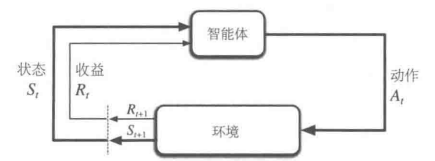
\includegraphics[width=0.5\textwidth]{Markov} 
\caption[马尔可夫决策过程]{马尔可夫决策过程}
\end{figure}

\begin{itemize}
\item 动作(A):智能体做出的选择,集合构成动作空间。
\item 状态(S):选择的基础,集合构成状态空间。
\item 收益(R):目标。
\end{itemize}
%------------------------------------------------
\paragraph{马尔可夫性(Markov Property)}~\\

未来状态仅依赖于当前状态,而独立于过去状态,即“无记忆性”。

$ S_t,R_t $只依赖于$ S_{t - 1},A_{t - 1} $,服从离散概率分布$ p(s', r|s, a) \doteq \Pr\{S_t = s', R_t = r|S_{t - 1} = s, A_{t - 1} = a\} $,即$ S_t,R_t $所有可能组合的概率和为1。
%------------------------------------------------
\paragraph{状态转移}
当前状态和动作下,转移到某状态的概率,包括该状态下各可能收益情况:
$$
p(s'|s, a) \doteq \Pr\{S_t = s'|S_{t - 1} = s, A_{t - 1} = a\} = \sum_{r \in R} p(s', r|s, a)
$$

以下分别给出了期望收益,后者相较于前者,指定了未来状态:
\begin{align*}
r(s, a) &\doteq E[R_t|S_{t - 1} = s, A_{t - 1} = a] = \sum_{r \in R} r \sum_{s' \in S} p(s', r|s, a) \\
r(s, a, s') &\doteq E[R_t|S_{t - 1} = s, A_{t - 1} = a, S_t = s'] = \sum_{r \in R} r \frac{p(s', r|s, a)}{p(s'|s, a)}  
\end{align*}

\begin{figure}[H]
\centering
\subfloat[状态转移图(节点不能重复)]{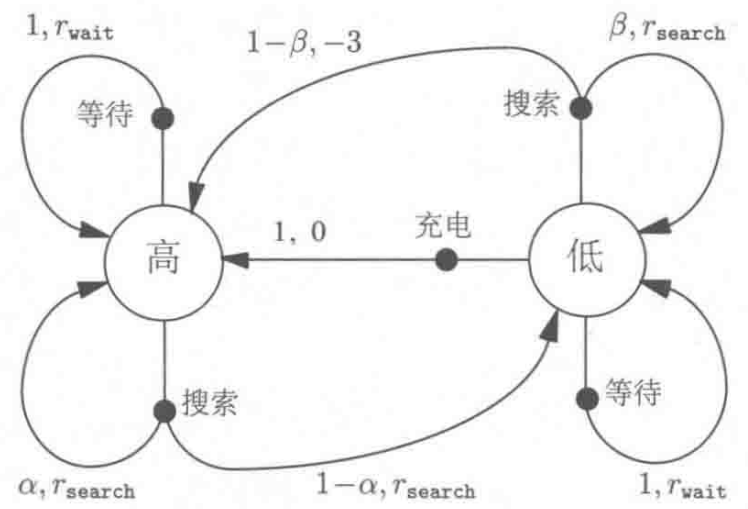
\includegraphics[width=.45\textwidth]{Transitions1}} \quad
\subfloat[状态转移表]{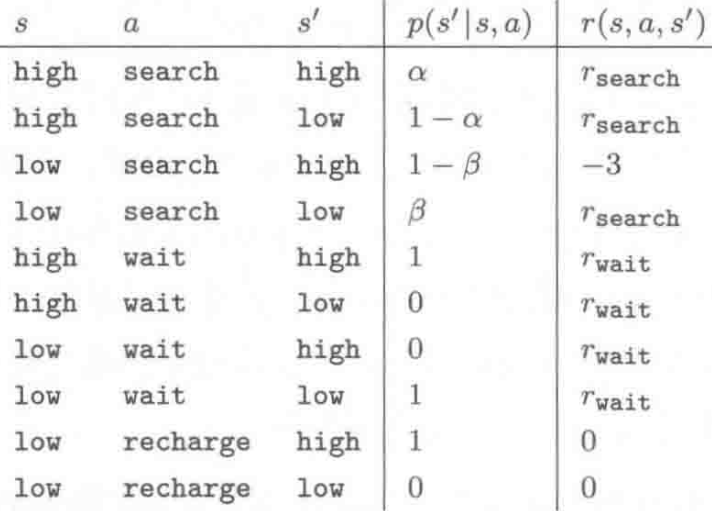
\includegraphics[width=.45\textwidth]{Transitions2}}
\caption[回收机器人状态转移]{回收机器人状态转移}
\end{figure}
%------------------------------------------------
\paragraph{构建要点}
\begin{itemize}
\item 确定动作、状态、收益。
\item 奖励与惩罚:相对的,可以全奖励或全惩罚。
\item 同一问题可能有多层次MDP。
\item 不同状态的可行动作设置:利用先验知识,人为排除愚蠢动作。
\end{itemize}
%------------------------------------------------
\subsection{元素}
%------------------------------------------------
\subsubsection{目标和收益}
\begin{itemize}
\item 目标:最大化长期累计收益。
\item 收益$ R_t $:不含先验知识,不为达到子目标而舍弃最终目标。
\item 回报$ G_t $:收益的总和。
\end{itemize}
%------------------------------------------------
\subsubsection{分幕回报与折扣}
\begin{itemize}
\item 分幕式任务:具有分幕重复特性,下一幕开始状态与上一幕终结状态无关。
$$ G_t = R_{t + 1} + R_{t + 2} + \cdots + R_T $$

其中$ T $是最终时刻,由其划分非终结状态集$ S $和所有状态集$ S^+ $。
\item 持续性任务:持续不断发生,不能自然分幕,最终时刻趋于无穷。
$$ G_t = R_{t + 1} + \gamma R_{t + 2} + \gamma^2 R_{t + 3} + \cdots = \sum_{k = 0}^{\infty} \gamma^k R_{t + k + 1} $$

其中,$ \gamma \in [0, 1] $是折扣率,其越大代表越考虑长期收益。
\item 统一表示:有限项终止后,状态持续转移回自己,相当于无限项。
$$ G_t \doteq \sum_{k = t + 1}^{T} \gamma^{k - t - 1} R_k $$
\end{itemize}
%------------------------------------------------
\subsubsection{策略和价值函数}
%------------------------------------------------
\paragraph{状态价值函数(策略$ \pi $下状态$ s $的价值)}
\begin{align*}
v_\pi(s) 
&\doteq E_\pi[G_t|S_t = s] = E_\pi[\sum_{k = 0}^{\infty} \gamma^k R_{t + k + 1}|S_t = s, A_t = a]\\
&= E_\pi[R_{t + 1} + \gamma G_{t+1}|S_t = s] \\
&= \sum_a \pi(a|s) \sum_{s'} \sum_r p(s', r|s, a)[r + \gamma E_\pi[G_{t + 1}|S_{t + 1} = s']] \\
&= \underbrace{\sum_a \pi(a|s) \sum_{s', r} p(s', r|s, a)[r + \gamma v_\pi(s')]}_{贝尔曼方程}, s \in S
\end{align*}
%------------------------------------------------
\paragraph{动作价值函数(策略$ \pi $下在状态$ s $采取动作$ a $的价值)}
$$ q_\pi(s, a) \doteq E_\pi[G_t|S_t = s, A_t = a] = E_\pi[\sum_{k = 0}^{\infty} \gamma^k R_{t + k + 1}|S_t = s, A_t = a] $$
%------------------------------------------------
\paragraph{回溯算法}
后继状态的价值信息回传给当前状态。

\begin{figure}[H]
\centering 
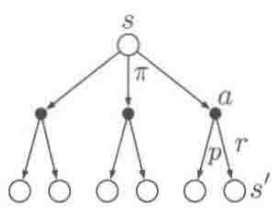
\includegraphics[width=0.3\textwidth]{DP} 
\caption[DP回溯图]{DP回溯图(节点可以重复)}
\end{figure}
%------------------------------------------------
\paragraph{最优策略}~\\

价值函数定义了策略的偏序关系,最优策略存在且可能不唯一,它们共享最优价值函数:
$$ v_*(s) \doteq \max_{\pi} v_{\pi}(s) \quad q_*(s, a) \doteq \max_{\pi} q_{\pi}(s, a) $$

将前者代入后者,得到状态-动作二元组$ q_*(s, a) = E[R_{t + 1} + \gamma v_*(S_{t + 1}), S_t = s, A_t = a] $。
%----------------------------------------------------------------------------------------
\subsection{贝尔曼方程}\tip{贝尔曼方程}
%------------------------------------------------
\subsubsection{贝尔曼方程}
$$
v_\pi(s) = \sum_a \pi(a|s) \sum_{s', r} p(s', r|s, a) [r + \gamma v_\pi(s')]
$$

可化简为$ v = r_\pi + \gamma P_\pi v $,其说明一个状态依赖其他状态值。
%------------------------------------------------
\subsubsection{贝尔曼最优方程}
作为一个方程组,方程数量对应状态数,如环境的动态变化特性$ p $已知,并具有马尔可夫性,则可以求解。但一般难以满足,且计算资源有限,求解近似解。
%------------------------------------------------
\paragraph{形式}
\begin{align*}
v_*(s) 
&= \max_{a \in A(s)} q_{\pi_*}(s, a) \\
&= \max_a E[R_{t + 1} + \gamma v_*(S_{t + 1})  S_t = s, A_t = a] \\
&= \max_a \sum_{s', r} p(s', r|s, a)[r + \gamma v_*(s')] \\
q_*(s, a) 
&= E[R_{t + 1} + \gamma \max_{a'} q_*(S_{t + 1}, a')  S_t = s, A_t = a] \\
&= \sum_{s', r} p(s', r|s, a)[r + \gamma \max_{a'} q_*(s', a')]
\end{align*}

\begin{figure}[H]
\centering 
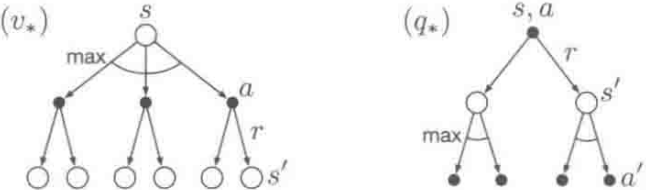
\includegraphics[width=0.7\textwidth]{DPbest} 
\caption[DP回溯图的两种形式(最优)]{DP回溯图的两种形式(最优)}
\end{figure}
%------------------------------------------------
\paragraph{描述方式}
\begin{itemize}
\item 元素:$ v(s) = \max_{\pi} \sum_{s \in S}\pi(a|s)q(s,a) $。
\item 矩阵向量:$ v = \max_{\pi} (r_\pi + \gamma P_\pi v) $。
\end{itemize}
%------------------------------------------------
\paragraph{求解}
伸缩映射性,见\ref{sec:Scalability Mapping}。\label{sec:Scalability Mapping back}
%------------------------------------------------
\paragraph{贪婪最优策略}
最优策略下,各状态价值一定等于其下最优动作的期望回报,可使用贪心策略求取(证明:凸组合最大值为最大一项)。
$$
\pi^*(a|s) = 
\begin{cases}
1, & a = a^*(s), \\
0, & a \neq a^*(s).
\end{cases}
$$

其中$ a^*(s) = argmax_a q^*(a, s), q^*(s, a) \doteq \sum_{r \in R} p(r|s, a) r + \gamma \sum_{s' \in S} p(s'|s, a) v^*(s') $。
%----------------------------------------------------------------------------------------
\section{动态规划(Dynamic Programming,DP):期望更新}
使用价值函数来结构化组织最优策略搜索,将贝尔曼方程转化成近似逼近理想价值函数的递归更新公式。
%------------------------------------------------
\subsection{策略迭代}\tip{策略迭代(算法)}
反复进行策略评估和策略迭代,得到改进的价值函数估计和策略,最后收敛到最优,收敛较快。
%------------------------------------------------
\paragraph{策略评估(PE)}
计算策略$ \pi $的状态价值函数$ v_{\pi_k} = r_{\pi_k} + \gamma P_{\pi_k}v_{\pi_k} $。
\begin{itemize}
\item 直接求解,$ v_{\pi_k} = (I - \gamma P_{\pi_k})^{-1} r_{\pi_k} $。
\item 迭代求解,$ v_{\pi_k}^{(j + 1)} = r_{\pi_k} + \gamma P_{\pi_k} v_{\pi_k}^{(j)}, j = 0, 1, 2, \dots $。
\end{itemize}
\begin{enumerate}
\item 期望更新:基于后继可能状态的期望值。
\item 截断策略评估:不需要策略评估完全收敛。
\end{enumerate}
%------------------------------------------------
\paragraph{策略改进(PI)}
$ \forall s \in S, q_{\pi}(s, \pi'(s)) = v_{\pi'}(s) \geq v_{\pi}(s) $,则称$ \pi' $优于或等于$ \pi $。根据原策略的价值函数,利用贪心方法构造新的策略,其一定不差于原策略。对于确定性策略和随机策略都成立。
$$ \pi_{k + 1} = argmax_{\pi}(r_{\pi} + \gamma P_{\pi}v_{\pi_k}) $$
%------------------------------------------------
\paragraph{策略迭代算法}
\begin{itemize}
\item 阈值$ \theta > 0 $确定估计精度
\item $ \forall s \in S $,任意初始化$ v(s) \in R, \pi(s)\in A(s) $
\item 策略评估:$ |v_{\pi_k}^{(j + 1)} - v_{\pi_k}^{(j)}| $大于阈值时:
\begin{itemize}
\item $ \forall s \in S $,$ v_{\pi_k}^{(j + 1)}(s) = \sum_a \pi_k(a|s)[\sum_r p(r|s, a)r + \gamma \sum_{s'}p(s'|s ,a)v_{\pi_k}^{(j)}(s')] $
\end{itemize}
\item 策略改进:
\begin{itemize}
\item  $ |v_{\pi_k}^{(j + 1)} - v_{\pi_k}^{(j)}| $大于阈值时:
\begin{itemize}
\item $ \forall s \in S $:
\begin{itemize}
\item $ \forall a \in A(s), q_{\pi_k}(s, a) = \sum_r p(r|s, a)r + \gamma \sum_{s'} p(s'|s, a)v_{\pi_k}(s') $。$ a^*_k(s) = argmax_a q_{\pi_k}(a, s) $
\end{itemize}
\end{itemize}
\item 如改进后策略不变则终止,改变则再次进行策略评估。(为防止在多个最优结果间摇摆,需额外判断)
\end{itemize}
\end{itemize}
%------------------------------------------------
\subsection{值迭代}\tip{值迭代(算法)}
只进行一次策略评估的遍历,对每个状态更新一次,结合了策略改进和极端策略评估。
更新公式如下:
$$
v_{k + 1}(s) = \max_a \sum_{s', r} p(s', r|s, a)[r + \gamma v_k(s')]
$$
%------------------------------------------------
\paragraph{策略更新(PU)}
$ \pi_{k + 1} = argmax_{\pi}(r_{\pi} + \gamma P_{\pi}v_k) $,贪婪选取$ a^*_k(s) = argmax_a q_k(a, s) $。
%------------------------------------------------
\paragraph{价值更新(VU)}
$ v_{k + 1} = r_{\pi_{k + 1}} + \gamma P_{\pi_{k + 1}}v_k = max_a q_k(a, s) $。
%------------------------------------------------
\paragraph{值迭代算法}
\begin{itemize}
\item 参数:阈值$ \theta > 0 $确定估计精度
\item $ \forall s \in S^+ $,任意初始化$ v(s) $,其中$ v(\text{终止}) = 0 $
\item 当$ |v_{k + 1} - v_k| > \theta $时:
\begin{itemize}
\item $ \forall s \in S $:
\begin{itemize}
\item $ \forall a \in A(s) $:
\begin{itemize}
\item $ q_k(s, a) = \sum_r p(r|s, a)r + \gamma \sum_{s'} p(s'|s, a)v_k(s') $
\item $ a^*_k(s) = \arg\max_a q_k(s, a) $
\item 策略更新:若$ a = a^*_k $且$ \pi_{k + 1}(a|s) = 0 $,则令$ \pi_{k + 1}(a|s) = 1 $
\item 价值更新:$ v_{k + 1}(s) = \max_a q_k(s, a) $
\end{itemize}
\end{itemize}
\end{itemize}
\item 输出策略$ \pi(s) = \arg\max_a \sum_{s',r}p(s',r|s,a)[r + \gamma V(s')] $
\end{itemize}
%------------------------------------------------
\subsection{其他内容}
%------------------------------------------------
\paragraph{异步动态规划}
使用任意可用状态值,以任意顺序更新,避免遍历更新,以减小计算量。
%------------------------------------------------
\paragraph{广义策略迭代(GPI)}
策略评估和策略改进以更细粒度进行交替,可视为竞争与合作。
%------------------------------------------------
\paragraph{动态规划的效率}
动态规划的时间复杂度是动作与状态数量的多项式级,在面对维度灾难时,优于线性规划和直接搜索。
%----------------------------------------------------------------------------------------
\section{蒙特卡洛(Monte Carlo,MC):采样更新}\tip{蒙特卡洛}
针对分幕式任务,不需要先验知识,即状态转移律(环境动态变化规律),通过多幕采样数据解决问题。
%------------------------------------------------
\paragraph{状态价值估计}
给定的一幕中,指定状态的一次出现叫做对其的一次访问(visit),第一次出现为首次访问。使用首次访问(first visit)和每次访问(every visit)的两种算法对一幕数据的使用程度不同,但当访问次数趋于无穷时,回报收敛到$ v_{\pi}(s) $。

\begin{figure}[H]
\centering 
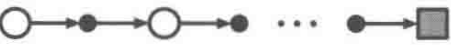
\includegraphics[width=0.3\textwidth]{MC} 
\caption[MC回溯图]{MC回溯图}
\end{figure}

动态规划的回溯图显示了一步的所有转移,而蒙特卡洛的回溯图显示一幕所有采样到的转移。
%------------------------------------------------
\paragraph{幕长}
靠近目标的状态比远离目标的状态更早具有非零值,幕长应足够长,无需无限长。
%------------------------------------------------
\paragraph{优势}
\begin{itemize}
\item 不需要环境动态特性模型。
\item 对每个状态的估计是独立的,可聚焦于状态子集,无需考虑其他状态。
\item 可从实际经历和模拟经历中学习。
\item 无马尔可夫性时性能损失较小。
\end{itemize}
%------------------------------------------------
\subsection{相关技术}
%------------------------------------------------
\subsubsection{柔性策略}
采取任何动作的概率都为正。
\begin{enumerate}
\item 试探性出发(ES):为采样部分无法正常获得的状态-动作二元组,可设定所有二元组都有概率作为起始。满足充分探索的理论要求,但实际中很难实现。
\end{enumerate}
%------------------------------------------------
\subsubsection{重要度采样}\tip{重要度采样}
计算回报时,对轨迹在目标策略和行为策略中出现的相对概率进行加权:
$$
\rho_{t:T - 1} = \Pi_{k = t}^{T - 1} \frac{\pi(A_k|S_k)}{b(A_k|S_k)}, \text{(约去相同的转移概率)}
$$
\begin{itemize}
\item 普通重要度采样:$ V(s) \doteq \frac{\sum_{t \in \tau(s)} \rho_{t:T(t) - 1}G_t}{|\tau(s)|} $,无偏但无界。
\item 加权重要度采样:$ V(s) \doteq \frac{\sum_{t \in \tau(s)} \rho_{t:T(t) - 1}G_t}{\sum_{t \in \tau(s)} \rho_{t:T(t) - 1}} $,有偏但偏差值渐近收敛。
\end{itemize}
%------------------------------------------------
\paragraph{减小方差的方法}
\begin{itemize}
\item 折扣敏感:把折扣率$ \gamma $视作幕终止的概率,得到第$ n $步终止的无折扣部分回报$ \sum_{i = 1}^n R_{t + i} $,即平价部分回报。全回报$ G_t = \sum_{i = 1}^{T - t} \gamma^{i - 1}R_{t + i} $可视为各平价部分回报的加权和,即该步截止得到的回报与概率之积的和。适用于普通重要度采样和加权重要度采样。
\item 每次决策型:$ E[\rho_{t:T - 1}G_t] = E[\tilde{G_t}] = E[\sum_{i = 1}^{T - t} \gamma^{i - 1} \rho_{t:t + i - 1}R_{t + i}] $。适用于普通重要度采样。
\end{itemize}
%------------------------------------------------
\subsubsection{增量式更新}
\begin{align*}
V_{n + 1} &\doteq V_n + \frac{W_n}{C_n}[G_n - V_n] \\
C_{n + 1} &\doteq C_n + W_{n + 1}
\end{align*}

其中,$ W_i $是随机权重,$ C_i $是其累加和。
%------------------------------------------------
\subsection{on-policy(同轨)}\tip{on-policy(算法)}
采样并改进相同策略。
%------------------------------------------------
\paragraph{on-policy算法}
\begin{itemize}
\item 参数:$ \epsilon > 0 $
\item 初始化:
\begin{itemize}
\item $ \forall s \in S, a \in A(s) $,任意初始化$ Q(s,a) \in R $,初始化$ Returns(s,a) $为空列表
\item $ \epsilon $-greedy初始化策略$ \pi $
\end{itemize}
\item 循环(对每幕):
\begin{itemize}
\item 根据$ \pi $生成一幕序列:$ S_0,A_0,R_1,S_1,A_1,R_2,\dots,S_{T - 1},A_{T - 1},R_T $
\item $ G = 0 $
\item 循环(对每步):$ t = T - 1, T - 2, \dots, 0 $
\begin{itemize}
\item $ G = \gamma G + R_{t + 1} $ 
\item 未出现过的$ S_t $,将$ G $加入$ Returns(S_t,A_t) $,$ Q(S_t,A_t) = \text{average}(Returns(S_t,A_t)) $
\item $ A^* = \arg \max_a Q(S_t,a) $
\item $ \forall a \in A(S_t) $,$ \pi(a|S_t) $由$ \epsilon $-greedy选取
\end{itemize}
\end{itemize}
\end{itemize}
%------------------------------------------------
\subsection{off-policy(离轨)}\tip{off-policy(算法)}
%------------------------------------------------
采样与改进不同策略,前者称为行为策略$ b $(保证对所有可能动作的采样),后者称为目标策略$ \pi $,可视为特殊的离轨。
%------------------------------------------------
\paragraph{off-policy算法}
\begin{itemize}
\item 初始化:$ \forall s \in S, a \in A(s), Q(s,a) \in R, C(s,a) = 0, \pi(s) = \arg \max_a Q(s,a) $
\item 循环(对每幕):
\begin{itemize}
\item $ b $为任意柔性策略
\item 根据$ b $生成一幕序列:$ S_0,A_0,R_1,S_1,A_1,R_2,\dots,S_{T - 1},A_{T - 1},R_T $
\item $ G = 0 $
\item $ W = 1 $
\item 循环(对每步):$ t = T - 1, T - 2, \dots, 0 $
\begin{itemize}
\item $ G = \gamma G + R_{t + 1} $ 
\item $ C(S_t,A_t) = C(S_t,A_t) + W $
\item $ Q(S_t,A_t) = Q(S_t,A_t) + \frac{W}{C(S_t,A_t)}[G - Q(S_t,A_t)] $
\item $ \pi(S_t) = \arg \max_a Q(S_t,a) $
\item 如果$ A_t \neq \pi(S_t) $,退出内层循环
\item 否则,$ W = W\frac{1}{b(A_t|S_t)} $
\end{itemize}
\end{itemize}
\end{itemize}

潜在问题:贪心行为普遍,只会从幕的尾部学习;贪心行为不普遍,学习速度较慢。
%----------------------------------------------------------------------------------------
\section{时序差分(Temporal Difference,TD):采样更新}
\tip{时序差分(TD(0)算法)}
TD可直接从与环境的互动中获取信息,不需要构建环境动态特性模型,同时运用自举思想,可基于已得到的其他状态的估计值来更新当前状态的价值函数,相当于同时结合了DP和MC的优点。
%------------------------------------------------
\subsection{TD(0)}
TD(0)的更新公式为:
$$
V_{t + 1}(S_t) = V_t(S_t) + \alpha_t(S_t)[R_{t + 1} + \gamma V_t(S_{t + 1}) - V_t(S_t)]
$$
\begin{itemize}
\item TD误差:$ [R_{t + 1} + \gamma V_t(S_{t + 1}) - V_t(S_t)] $。
\item TD目标:$ R_{t + 1} + \gamma V_t(S_{t + 1}) $
\end{itemize}

MC必须等到幕尾才能确定增量,更新$ G_t $;而TD只需等到下一时刻,更新$ R_{t + 1} + \gamma V(S_{t + 1}) $。

MC误差可写成TD误差之和$ G_t - V(S_t) = \sum_{k = t}^{T - 1} \gamma^{k - t} \delta_k $,其在步长较小时成立。

\begin{figure}[H]
\centering
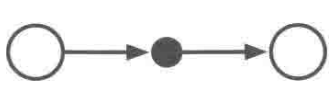
\includegraphics[width=0.2\textwidth]{TD}
\caption[TD回溯图]{TD回溯图}
\end{figure}
%------------------------------------------------
\paragraph{TD(0)算法}
\begin{itemize}
\item 输入:待评估策略$ \pi $
\item 参数:步长$ \alpha \in (0,1] $
\item $ \forall s \in S^+ $,任意初始化$ V(s) $,$ V(\text{终止状态}) = 0 $
\item 对每幕:
\begin{itemize}
\item 初始化$ S $
\item 对每步:
\begin{itemize}
\item $ A $为策略$ \pi $在状态$ S $下做出的决策动作
\item 观察$ A $带来的$ R, S' $
\item $ V(S) = V(S) + \alpha[R + \gamma V(S') - V(S)] $
\item $ S = S' $
\end{itemize}
\item 直到$ S $为终止状态
\end{itemize}
\end{itemize}
%------------------------------------------------
\paragraph{随机游走}
在随机任务实践中,TD(0)的收敛速度要比常量$ \alpha $MC快。这是因为前者的最优性与预测回报更相关,找出的是完全符合马尔可夫过程模型的最大似然估计参数,收敛到确定性等价估计;而后者只在有限方面最优,找出的是最小化训练集均方误差的估计。
%------------------------------------------------
\paragraph{批量更新}
价值函数根据增量和改变,在处理整批数据后才更新。
%------------------------------------------------
\subsection{Sarsa(on-policy-TD)}\tip{Sarsa(算法)}
Sarsa是TD算法的动作值版本:
$$
Q_{t + 1}(S_t, A_t) = Q_t(S_t, A_t) + \alpha_t[R_{t + 1} + \gamma Q_t(S_{t + 1}, A_{t + 1}) - Q_t(S_t, A_t)]
$$

其中,$ Q(S_{t + 1}, A_{t + 1}) - Q(S_t, A_t) $是自学习。

\begin{figure}[H]
\centering
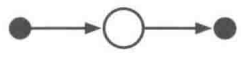
\includegraphics[width=0.2\textwidth]{Sarsa}
\caption[Sarsa回溯图]{Sarsa回溯图}
\end{figure}
%------------------------------------------------
\paragraph{Sarsa算法}
\begin{itemize}
\item 参数:步长$ \alpha \in (0,1] $,$ \epsilon > 0 $
\item $ \forall s \in S^+ $,任意初始化$ Q(s,a) $,$ Q(\text{终止状态,}) = 0 $
\item 对每幕:
\begin{itemize}
\item 初始化$ S $
\item 使用从$ Q $得到的策略,在$ S $处选择$ A $
\item 对每步:
\begin{itemize}
\item 执行$ A $,观察$ R,S' $
\item 使用从$ Q $得到的策略,在$ S' $处选择$ A' $
\item $ Q(S, A) = Q(S, A) + \alpha [R + \gamma Q(S', A') - Q(S, A)] $
\item $ S = S', A = A' $
\end{itemize}
\item 直到$ S $为终止状态
\end{itemize}
\end{itemize}
%------------------------------------------------
\paragraph{期望Sarsa}\tip{期望Sarsa}
$$
Q_{t + 1}(S_t, A_t) = Q_t(S_t, A_t) + \alpha_t[R_{t + 1} + \gamma \sum_a \pi(a|S_{t + 1}) Q_t(S_{t + 1}, a) - Q_t(S_t, A_t)]
$$

期望Sarsa相较Sarsa,虽然计算复杂,但是消除了随机选择带来的方差。$ \alpha $的选择对二者有一定影响,尤其在长期稳态性能上。生成策略可以基于相同或不同策略,即离轨或在轨是可变的。基于此,Q-learning可视为期望Sarsa的一个特例。
\begin{figure}[H]
\centering
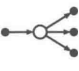
\includegraphics[width=0.2\textwidth]{eSarsa}
\caption[期望Sarsa回溯图]{期望Sarsa回溯图}
\end{figure}
%------------------------------------------------
\subsection{Q-learning(off-policy-TD)}\tip{Q-learning(算法)}
Q-learning旨在求解动作值表示的贝尔曼最优方程。
$$
Q_{t + 1}(S_t, A_t) = Q_t(S_t, A_t) + \alpha_t[R_{t + 1} + \gamma \max_a Q_t(S_{t + 1}, a) - Q_t(S_t, A_t)]
$$

$ \max_a Q(S_{t + 1}, a) - Q(S_t, A_t) $是更丰富地学习。

\begin{figure}[H]
\centering
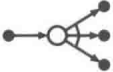
\includegraphics[width=0.2\textwidth]{Q}
\caption[Q-learning回溯图]{Q-learning回溯图}
\end{figure}
%------------------------------------------------
\paragraph{Q-learning算法}
\begin{itemize}
\item 参数:步长$ \alpha \in (0,1] $,$ \epsilon > 0 $
\item $ \forall s \in S^+, a \in A(s) $,任意初始化$ Q(s,a) $,$ Q(\text{终止状态,}) = 0 $
\item 对每幕:
\begin{itemize}
\item 初始化$ S $
\item 对每步:
\begin{itemize}
\item 使用从$ Q $得到的策略,在$ S $处选择$ A $
\item 执行$ A $,观察$ R,S' $
\item $ Q(S, A) = Q(S, A) + \alpha [R + \gamma \max_a Q(S', a) - Q(S, A)] $
\item $ S = S' $
\end{itemize}
\item 直到$ S $为终止状态
\end{itemize}
\end{itemize}
%------------------------------------------------
\paragraph{双Q-learning}\tip{双Q-learning(算法)}
\begin{itemize}
\item 最大化偏差:贪心策略和柔性策略都在隐式估计最大值,会产生正偏差,这会致使回报值偏离,带来选择一些明显错误的决策。
\item 双学习:划分样本,学习两个独立的估计$ Q_1(a),Q_2(a) $,确定动作$ A* = argmax_a Q_1(a) $,再计算价值的估$ Q_2(A*) = Q_2(argmax_a Q_1(a)) $,后者是无偏的(可以交换再来一次)。需要双倍内存,但是计算量维持。
\item 后位状态:利用先验知识,知晓动作后的状态,并有后位状态价值函数。在后位状态相同的时候,可以迁移,减少计算量。
\end{itemize}
%------------------------------------------------
\paragraph{双Q-learning算法}
\begin{itemize}
\item 参数:步长$ \alpha \in (0,1] $,$ \epsilon > 0 $
\item $ \forall s \in S^+, a \in A(s) $,任意初始化$ Q_1(s,a),Q_2(s,a) $,$ Q(\text{终止状态,}) = 0 $
\item 对每幕:
\begin{itemize}
\item 初始化$ S $
\item 对每步:
\begin{itemize}
\item 基于$ Q_1 + Q_2 $,使用策略在$ S $处选择$ A $
\item 执行$ A $,观察$ R,S' $
\item 分别以$ 0.5 $的概率执行:
\begin{itemize}
\item $ Q_1(S, A) = Q_1(S, A) + \alpha [R + \gamma Q_2(S', \arg \max_a Q_1(S',a)) - Q_1(S, A)] $
\item $ Q_2(S, A) = Q_2(S, A) + \alpha [R + \gamma Q_1(S', \arg \max_a Q_2(S',a)) - Q_2(S, A)] $
\end{itemize}
\item $ S = S' $
\end{itemize}
\item 直到$ S $为终止状态
\end{itemize}
\end{itemize}
%------------------------------------------------
\subsection{DP、MC、TD总结对比}\tip{DP、MC、TD总结对比}
\begin{figure}[H]
\centering
\subfloat[DP]{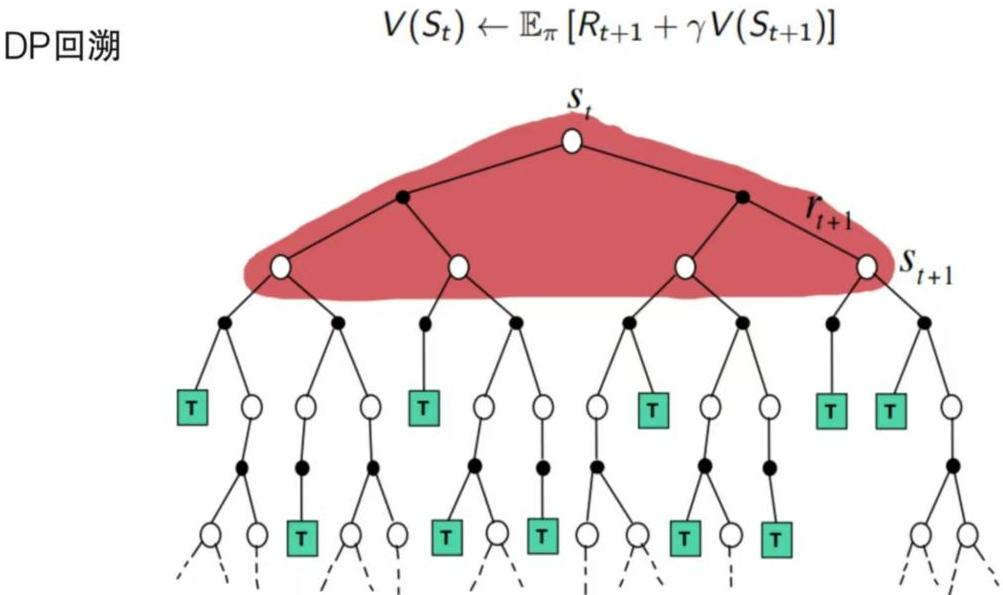
\includegraphics[width=.3\textwidth]{compare_DP}} \quad
\subfloat[MC]{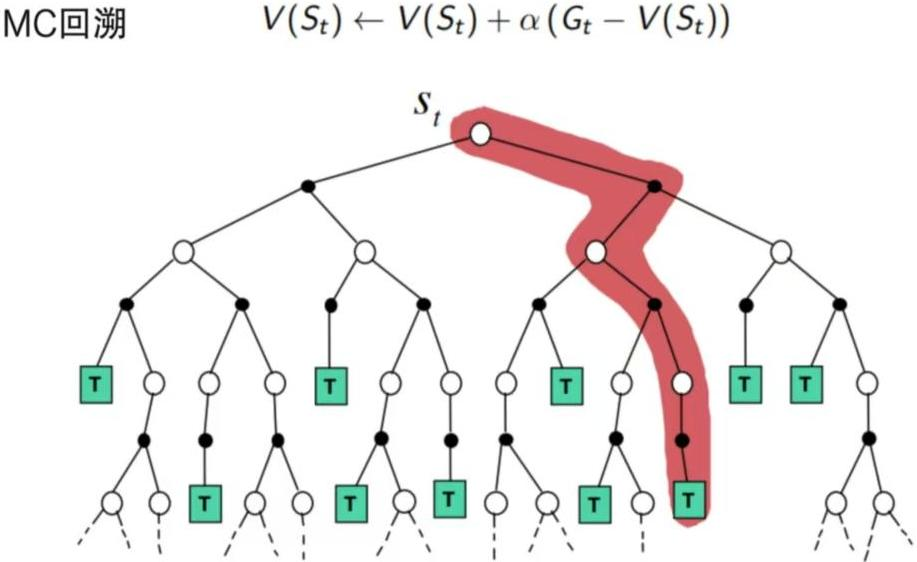
\includegraphics[width=.3\textwidth]{compare_MC}} \quad
\subfloat[TD]{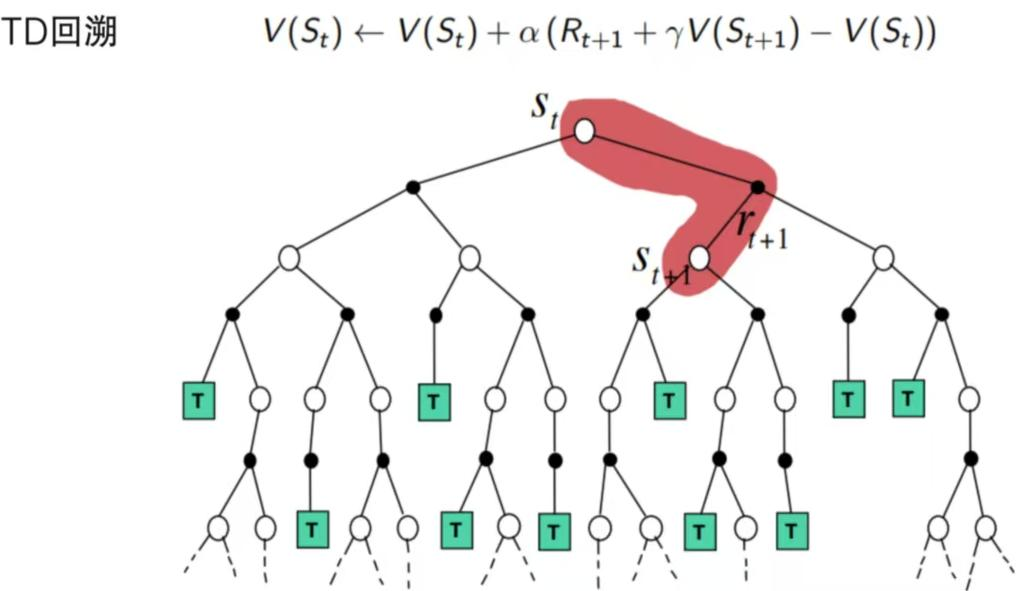
\includegraphics[width=.3\textwidth]{compare_TD}}
\caption[DP、MC、TD对比]{DP、MC、TD对比}
\end{figure}
统一格式:
$$ Q_{t + 1}(S_t, A_t) = Q_t(S_t, A_t) + \alpha_t(S_t, A_t)[\bar{q}_t - Q_t(S_t, A_t)] $$

\begin{figure}[H]
\centering
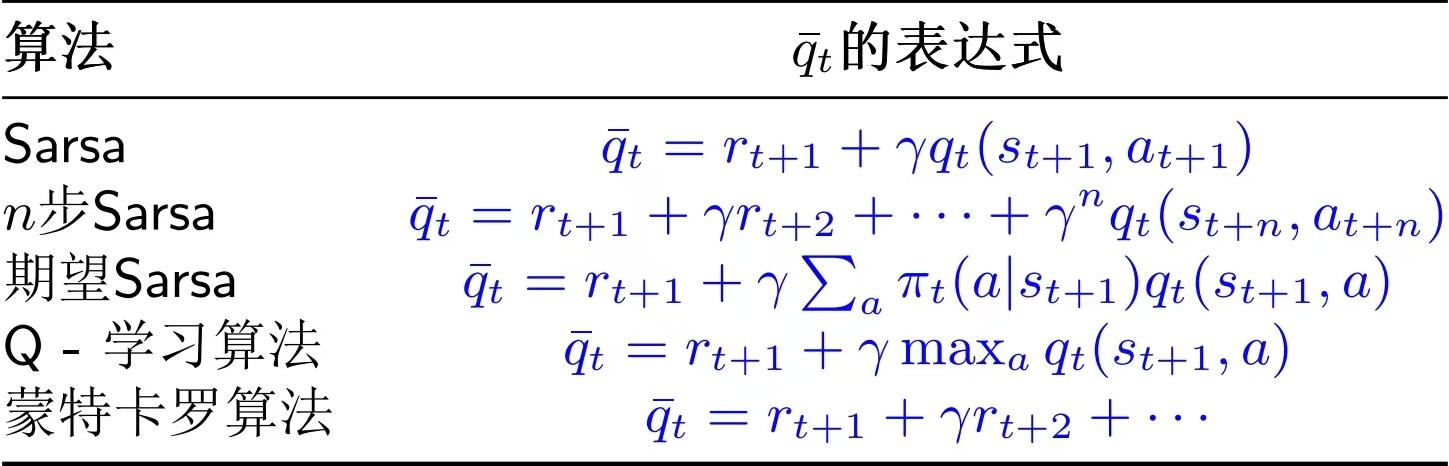
\includegraphics[width=0.6\textwidth]{all_q}
\caption[算法表达式总结]{算法表达式总结}
\end{figure}
%----------------------------------------------------------------------------------------
\section{n步自举法}
%------------------------------------------------
\subsection{n步TD}\tip{n步TD(算法)}
n步TD作为MC和TD的一般推广,在两种极端方法间找到了性能更好的平衡点。n步TD在$ n $步后进行更新,截断得到$ n $步回报。
$$ G_{t:t + n} \doteq R_{t + 1} + \gamma R_{t + 2} + \dots + \gamma^{n - 1} R_{t + n} + \gamma^n V_{t + n - 1}(S_{t + n}) $$

其中$ V_{t + n}(S_t) \doteq V_{t + n - 1}(S_t) + \alpha[G_{t:t + n} - V_{t + n - 1}(S_t)] $。
%------------------------------------------------
\paragraph{n步TD算法}
\begin{itemize}
\item 输入:待评估策略$ \pi $
\item 参数:步长$ \alpha \in (0,1] $,$ n \in N_+ $
\item $ \forall s \in S $,任意初始化$ V(s) $
\item 对每幕:
\begin{itemize}
\item 初始化$ S_0 $,其非终止状态
\item $ T = \infty $
\item 对$ t = 0, 1, 2, \dots $:
\begin{itemize}
\item $ t < T $时:
\begin{itemize}
\item 根据$ \pi(\cdot|S_t) $采取策略
\item 观察$ R_{t + 1}, S_{t + 1} $
\item 如果$ S_{t + 1} $是终止状态,则$ T = t + 1 $
\end{itemize}
\item $ \tau = t - n + 1 $
\item 如果$ \tau \geq 0 $:
\begin{itemize}
\item $ G = \sum_{i = \tau + 1}^{\min(\tau + n, T)} \gamma^{i - \tau - 1}R_i $
\item 如果$ \tau + n < T $,$ G = G + \gamma^n V(S_{\tau + n}) $
\item $ V(S_{\tau}) = V(S_{\tau}) + \alpha[G - V(S_{\tau})] $
\end{itemize}
\end{itemize}
\item 直到$ \tau = T - 1 $
\end{itemize}
\end{itemize}
%------------------------------------------------
\subsection{n步Sarsa}\tip{n步Sarsa(算法)}
n步Sarsa统一了Sarsa和MC,其节点转移全部基于采样得到的单独路径:
$$ Q_{t + n}(S_t, A_t) \doteq Q_{t + n - 1}(S_t, A_t) + \alpha [G_{t:t + n} - Q_{t + n - 1}(S_t, A_t)] $$

n步期望Sarsa只对最后一个状态到动作的转移展开:
$$ G_{t:t + n} \doteq R_{t + 1} + \gamma R_{t + 2} + \dots + \gamma^{n - 1} R_{t + n} + \gamma^n \bar{V}_{t + n - 1}(S_{t + n}) $$

\begin{figure}[H]
\centering
\subfloat[n步Sarsa]{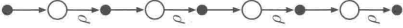
\includegraphics[width=.6\textwidth]{nSarsa}} \\
\subfloat[n步期望Sarsa]{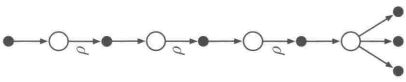
\includegraphics[width=.6\textwidth]{neSarsa}}
\caption[n步Sarsa回溯图]{n步Sarsa回溯图}
\end{figure}
%------------------------------------------------
\paragraph{n步Sarsa算法}
\begin{itemize}
\item 参数:步长$ \alpha \in (0,1] $,$ \epsilon > 0 $,$ n \in N_+ $
\item $ \forall s \in S, a \in A $,任意初始化$ Q(s, a) $
\item 初始化$ \pi $
\item 对每幕:
\begin{itemize}
\item 初始化$ S_0 $,其非终止状态
\item 根据$ \pi(\cdot|S_0) $选取$ A_0 $
\item $ T = \infty $
\item 对$ t = 0, 1, 2, \dots $:
\begin{itemize}
\item $ t < T $时:
\begin{itemize}
\item 采取$ A_t $,观察$ R_{t + 1}, S_{t + 1} $
\item 如果$ S_{t + 1} $是终止状态,则$ T = t + 1 $;否则根据$ \pi(\cdot|S_{t + 1}) $选取$ A_{t + 1} $
\end{itemize}
\item $ \tau = t - n + 1 $
\item 如果$ \tau \geq 0 $:
\begin{itemize}
\item $ G = \sum_{i = \tau + 1}^{\min(\tau + n, T)} \gamma^{i - \tau - 1}R_i $
\item 如果$ \tau + n < T $,$ G = G + \gamma^n Q(S_{\tau + n}, A_{\tau + n}) $
\item $ Q(S_{\tau},A_{\tau}) = Q(S_{\tau},A_{\tau}) + \alpha[G - Q(S_{\tau},A_{\tau})] $
\end{itemize}
\end{itemize}
\item 直到$ \tau = T - 1 $
\end{itemize}
\end{itemize}
%------------------------------------------------
\subsection{n步off-policy}\tip{n步off-policy(算法)}
针对离线n步时序差分学习,有:
$$ V_{t + n}(S_t) \doteq V_{t + n - 1}(S_t) + \alpha \rho_{t:t + n - 1}[G_{t:t + n} - V_{t + n - 1}(S_t)] $$
其中,重要度采样率为目标策略和行为策略采取$ n $个动作的相对概率:
$$ \rho_{t:h} \doteq \prod_{k = t}^{\min(h, T - 1)} \frac{\pi(A_k|S_k)}{b(A_k|S_k)} $$
%------------------------------------------------
\paragraph{n步期望Sarsa-off-policy算法}
\begin{itemize}
\item 输入:行为策略$ b, b(a|s) > 0 $
\item 参数:步长$ \alpha \in (0,1] $,$ \epsilon > 0 $,$ n \in N_+ $
\item $ \forall s \in S, a \in A $,任意初始化$ Q(s, a) $
\item 初始化$ \pi $
\item 对每幕:
\begin{itemize}
\item 初始化$ S_0 $,其非终止状态
\item 根据$ b(\cdot|S_0) $选取$ A_0 $
\item $ T = \infty $
\item 对$ t = 0, 1, 2, \dots $:
\begin{itemize}
\item $ t < T $时:
\begin{itemize}
\item 采取$ A_t $,观察$ R_{t + 1}, S_{t + 1} $
\item 如果$ S_{t + 1} $是终止状态,则$ T = t + 1 $;否则根据$ b(\cdot|S_{t + 1}) $选取$ A_{t + 1} $
\end{itemize}
\item $ \tau = t - n + 1 $
\item 如果$ \tau \geq 0 $:
\begin{itemize}
\item $ \rho = \prod_{i = \tau + 1}^{\min(\tau + n - 1,T - 1)} \frac{\pi(A_i|S_i)}{b(A_i|S_i)} $
\item $ G = \sum_{i = \tau + 1}^{\min(\tau + n, T)} \gamma^{i - \tau - 1}R_i $
\item 如果$ \tau + n < T $,$ G = G + \gamma^n Q(S_{\tau + n}, A_{\tau + n}) $ 
\item $ Q(S_{\tau},A_{\tau}) = Q(S_{\tau},A_{\tau}) + \alpha \rho[G - Q(S_{\tau},A_{\tau})] $
\end{itemize}
\end{itemize}
\item 直到$ \tau = T - 1 $
\end{itemize}
\end{itemize}
%------------------------------------------------
\subsection{n步树回溯}\tip{n步树回溯(算法)}
%------------------------------------------------
\paragraph{带控制变量的每次决策模型}
为保证不被选择的动作不会因$ \rho_t = 0 $而回报为$ 0 $,使方差较大,采取以下n步回报离轨方法:
$$ G_{t:h} \doteq \rho_t (R_{t + 1} + \gamma G_{t + 1:h}) + (1 - \rho_t) V_{h - 1}(S_t) $$

其中$ (1 - \rho_t) V_{h - 1}(S_t) $称为控制变量,其能保证$ \rho_t = 0 $时估计值不收缩,但不会改变更新值的期望。

使用控制变量的离轨策略可以写为以下递归形式:
\begin{align*}
G_{t:h} 
&\doteq R_{t + 1} + \gamma[\rho_{t + 1} G_{t + 1:h} + \bar{V}_{h - 1}(S_{t + 1}) - \rho_{t + 1} Q_{h - 1}(S_{t + 1}, A_{t + 1})] \\
&= R_{t + 1} + \gamma \rho_{t + 1}[G_{t + 1:h} - Q_{h - 1}(S_{t + 1}, A_{t + 1})] + \gamma \bar{V}_{h - 1}(S_{t + 1})
\end{align*}
%------------------------------------------------
\paragraph{n步树回溯}
离轨因为所学内容相关性小,比同轨缓慢,一些方法可以缓解这一问题,比如不使用重要度采样的树回溯算法。相比于前面以沿途收益和底部节点估计价值为更新目标的算法,树回溯的更新源于整个树的动作价值估计,即各叶子节点的动作价值估计按出现概率加权。
单步回溯树:
$$ G_{t:t + 1} \doteq R_{t + 1} + \gamma \sum_{a} \pi(a|S_{t + 1}) Q_t(S_{t + 1}, a) $$

拓展到n步回溯树的递归形式,其对路径可能分支进行展开,不进行采样:
$$ G_{t:t + n} \doteq R_{t + 1} + \gamma \sum_{a \neq A_{t + 1}} \pi(a|S_{t + 1}) Q_{t + n - 1}(S_{t + 1}, a) + \gamma \pi(A_{t + 1}|S_{t + 1}) G_{t + 1:t + n} $$

\begin{figure}[H]
\centering
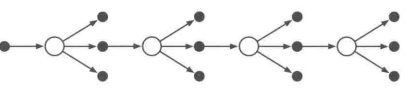
\includegraphics[width=0.6\textwidth]{ntree}
\caption[n步树回溯回溯图]{n步树回溯回溯图}
\end{figure}

这个目标可以用于n步Sarsa的动作价值更新。
%------------------------------------------------
\paragraph{n步树回溯算法}
\begin{itemize}
\item 参数:步长$ \alpha \in (0,1] $,$ n \in N_+ $
\item $ \forall s \in S, a \in A $,任意初始化$ Q(s, a) $
\item 初始化$ \pi $
\item 对每幕:
\begin{itemize}
\item 初始化$ S_0 $,其非终止状态
\item 根据$ S_0 $任意选取$ A_0 $
\item $ T = \infty $
\item 对$ t = 0, 1, 2, \dots $:
\begin{itemize}
\item $ t < T $时:
\begin{itemize}
\item 采取$ A_t $,观察$ R_{t + 1}, S_{t + 1} $
\item 如果$ S_{t + 1} $是终止状态,则$ T = t + 1 $;否则根据$ S_{t + 1} $选取$ A_{t + 1} $
\end{itemize}
\item $ \tau = t - n + 1 $
\item 如果$ \tau \geq 0 $:
\begin{itemize}
\item 如果$ t + 1 \geq T $,$ G = R_T $;否则$ G = R_{t + 1} + \gamma \sum_a \pi(a|S_{t + 1})Q(S_{t + 1},a) $
\item 循环$ k = \min(t, T - 1) $递减到$ \tau + 1 $,$ G = R_k + \gamma \sum_{a \neq A_k} \pi(a|S_k)Q(S_k,a) + \gamma \pi(A_k|S_k)G $
\item $ Q(S_{\tau},A_{\tau}) = Q(S_{\tau},A_{\tau}) + \alpha[G - Q(S_{\tau},A_{\tau})] $
\end{itemize}
\end{itemize}
\item 直到$ \tau = T - 1 $
\end{itemize}
\end{itemize}
%------------------------------------------------
\subsection{n步Q($ \sigma $)}\tip{n步Q($ \sigma $)(算法)}
结合采样的Sarsa和展开的树回溯,在每个状态由参数$ \sigma $决定是采样还是展开,即n步Q$ (\sigma) $算法,其将两种线性情况组合起来:
$$ G_{t:h} \doteq R_{t + 1} + \gamma (\sigma_{t + 1} \rho_{t + 1} + (1 - \sigma_{t + 1}) \pi(A_{t + 1}|S_{t + 1}))(G_{t + 1:h} - Q_{h - 1}(S_{t + 1}, A_{t + 1})) + \gamma \bar{V}_{h - 1}(S_{t + 1}) $$

\begin{figure}[H]
\centering
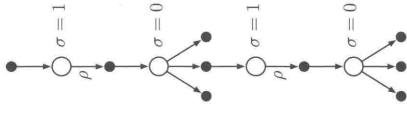
\includegraphics[width=0.6\textwidth]{Qsigma}
\caption[Q(sigma)回溯图]{Q(sigma)回溯图}
\end{figure}
%------------------------------------------------
\paragraph{n步Q($ \sigma $)-off-policy算法(n步Sarsa更新)}
\begin{itemize}
\item 输入:行为策略$ b, b(a|s) > 0 $
\item 参数:步长$ \alpha \in (0,1] $,$ \epsilon > 0 $,$ n \in N_+ $
\item $ \forall s \in S, a \in A $,任意初始化$ Q(s, a) $
\item 初始化$ \pi $
\item 对每幕:
\begin{itemize}
\item 初始化$ S_0 $,其非终止状态
\item 根据$ b(\cdot|S_0) $选取$ A_0 $
\item $ T = \infty $
\item 对$ t = 0, 1, 2, \dots $:
\begin{itemize}
\item $ t < T $时:
\begin{itemize}
\item 采取$ A_t $,观察$ R_{t + 1}, S_{t + 1} $
\item 如果$ S_{t + 1} $是终止状态,则$ T = t + 1 $;否则根据$ b(\cdot|S_{t + 1}) $选取$ A_{t + 1} $,选择$ \sigma_{t + 1} $,计算$ \rho_{t + 1} = \frac{\pi(A_{t + 1}|S_{t + 1})}{b(A_{t + 1}|S_{t + 1})} $
\end{itemize}
\item $ \tau = t - n + 1 $
\item 如果$ \tau \geq 0 $:
\begin{itemize}
\item $ G = 0 $
\item 循环$ k = \min(t, T - 1) $递减到$ \tau + 1 $:
\item $ k = T $,则$ G = R_T $;否则,$ \bar{V} = \sum_a \pi(a|S_k)Q(S_k,a) $。$ G = R_k + \gamma[\sigma_k \rho_k + (1 - \sigma_k)\pi(A_k|S_k)][G - Q(S_k,A_k)] + \gamma\bar{V} $
\item $ Q(S_{\tau},A_{\tau}) = Q(S_{\tau},A_{\tau}) + \alpha[G - Q(S_{\tau},A_{\tau})] $
\end{itemize}
\end{itemize}
\item 直到$ \tau = T - 1 $
\end{itemize}
\end{itemize}
%----------------------------------------------------------------------------------------
\section{基于表格型方法的规划和学习}
基于模型的方法(DP、启发式搜索)主要进行规划,无模型的方法(MC、TD)则主要进行学习,二者的核心都是价值函数的计算。
%------------------------------------------------
\subsection{模型和规划}
%------------------------------------------------
\paragraph{模型}
\begin{itemize}
\item 分布模型:生成所有可能的结果的描述与概率分布。
\item 样本模型:从所有可能中生成一个确定的结果,其通过概率分布采样得到。
\item 分布模型可以生成样本模型,但样本模型一般更容易获得。
\end{itemize}
%------------------------------------------------
\paragraph{规划}
\begin{itemize}
\item 规划:以环境模型为输入,生成或改进与其进行交互的策略。
\item 状态空间规划:在状态空间搜索最优策略。
\item 方案空间规划:进化算法、偏序规划。
\end{itemize}
%------------------------------------------------
\paragraph{统一的状态空间规划算法}
通过仿真经验的回溯操作计算价值函数,将其作为改善策略的中间步骤。
$$ \text{模型} \Longrightarrow \text{模拟经验} \overset{\text{回溯}}{\Longrightarrow} \text{价值函数} \Longrightarrow \text{策略} $$

各算法的差异集中在回溯操作、执行操作顺序、回溯信息保留时长上。极小步长适于大尺度规划问题。
%------------------------------------------------
\paragraph{随机采样单步表格型Q规划算法}
\begin{itemize}
\item 循环:
\begin{itemize}
\item 随机选择$ s \in S, a \in A(s) $
\item 采样$ (s, a) $的$ r,s' $
\item 规划:$ Q(s, a) = Q(s, a) + \alpha[r + \gamma \max_aQ(s', a) - Q(s, a)] $
\end{itemize}
\end{itemize}
%------------------------------------------------
\subsection{Dyna-Q}
学习和规划由相同算法完成,真实经验用于学习,模拟经验用于规划。
%------------------------------------------------
\paragraph{框架}
\begin{itemize}
\item 间接强化学习:更充分地利用有限经验,获得更好的策略,减少与环境的交互作用。
\item 直接强化学习:不受模型设计偏差影响。
\end{itemize}
%------------------------------------------------
\paragraph{表格型Dyna-Q算法}
\begin{itemize}
\item $ \forall s \in S, a \in A(s) $,初始化$ Q(s, a),Model(s, a) $(基于$ (s, a) $预测的后继状态和收益)
\item 循环:
\begin{itemize}
\item $ S $为当前状态,其非终止状态
\item 基于$ (S, Q) $选取$ A $
\item 采取$ A $,观察$ R,S' $
\item $ Q(s, a) = Q(s, a) + \alpha[R + \gamma \max_aQ(s', a) - Q(s, a)] $
\item $ Model(s, a) = R,S' $
\item 循环n次:
\begin{itemize}
\item 随机选择观测过的$ S $和其下采取过的$ A $
\item $ R,S' = Model(S, A) $
\item $ Q(s, a) = Q(s, a) + \alpha[R + \gamma \max_aQ(s', a) - Q(s, a)] $
\end{itemize}
\end{itemize}
\end{itemize}
%------------------------------------------------
\subsection{改进方法}
%------------------------------------------------
\paragraph{模型错误}
鼓励长期未出现过的动作,这些动作的模型可能是不正确的。通过鼓励试探所有可访问的状态转移,规避在次优解收敛。
%------------------------------------------------
\paragraph{优先遍历}
相比于均匀采样无长期收益的动作,集中更新有收益的动作会更有意义。反向聚焦提供了相应的思路。关联前导动作和前导状态,在后续动作有收益时先更新前导动作的价值,进行有效更新。按照价值改变多少对状态-动作二元组进行优先级排序,并由后至前反向传播出高影响序列。优先遍历为提高规划效率分配了计算量,但由于采用期望更新而在随机环境中有所局限。
%------------------------------------------------
\paragraph{确定性环境下的优先级遍历算法}
\begin{itemize}
\item $ \forall s \in S, a \in A(s) $,初始化$ Q(s, a),Model(s, a) $,初始化$ PQuene $为空
\item 循环:
\begin{itemize}
\item $ S $为当前状态,其非终止状态
\item 基于$ (S, Q) $选取$ A $
\item 采取$ A $,观察$ R,S' $
\item $ Model(s, a) = R,S' $
\item $ P = |R + \gamma \max_a Q(S',a) - Q(S,a)| $
\item $ P > 0 $将$ (S,A) $以优先级$ P $插入$ PQuene $
\item 循环n次($ PQuene $非空):
\begin{itemize}
\item $ S,A = PQuene(0) $ 
\item $ R,S' = Model(S, A) $
\item $ Q(s, a) = Q(s, a) + \alpha[R + \gamma \max_aQ(s', a) - Q(s, a)] $
\item 对可达$ S $的$ \bar{S},\bar{A} $进行上述迭代
\end{itemize}
\end{itemize}
\end{itemize}
%------------------------------------------------
\paragraph{轨迹采样}
借助模拟生成经验来进行回溯更新称为轨迹采样。同轨策略轨迹采样对于大尺度问题有一定优势,能够跳过无关状态,获得最优部分策略。

实时动态规划(RTDP)是价值迭代算法的同轨策略轨迹采样版本,属于异步DP。它可以在较少访问频率下为一些任务找到最优策略,并且产生轨迹所用的策略也会接近最优策略。
%------------------------------------------------
\paragraph{启发式搜索}
聚焦于当前状态。
%------------------------------------------------
\paragraph{预演算法}
作为MC的一个特例,通过平均多个起始于可能动作并遵循给定策略的模拟轨迹的回报来估计动作价值,可以改进预演策略的性能。

蒙特卡洛树搜索(MCTS)作为一种预演算法,通过累积蒙特卡洛模拟得到的价值估计来不停地将模拟导向高收益轨迹。其一次循环中包含选择、扩展、模拟、回溯四个步骤。
%------------------------------------------------
\subsection{总结对比}\tip{表格型方法总结对比}
\begin{minipage}{0.3\textwidth}
\paragraph{三个维度}   
\begin{itemize}
\item 更新
\item 自举程度
\item 同轨/离轨
\end{itemize}
\end{minipage}
\hfill
\begin{minipage}{0.6\textwidth}
\begin{figure}[H]
\centering
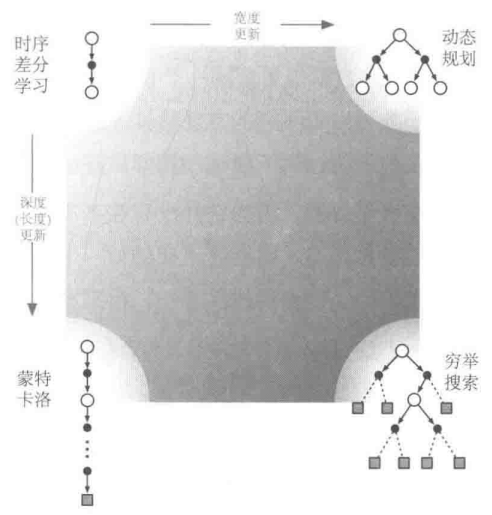
\includegraphics[width=\textwidth]{all}
\caption[表格型方法总结对比]{表格型方法总结对比}
\end{figure}
\end{minipage}
%------------------------------------------------
\paragraph{更新}
期望更新能产生更好的估计,但是需要更多的计算。

\begin{figure}[H]
\centering
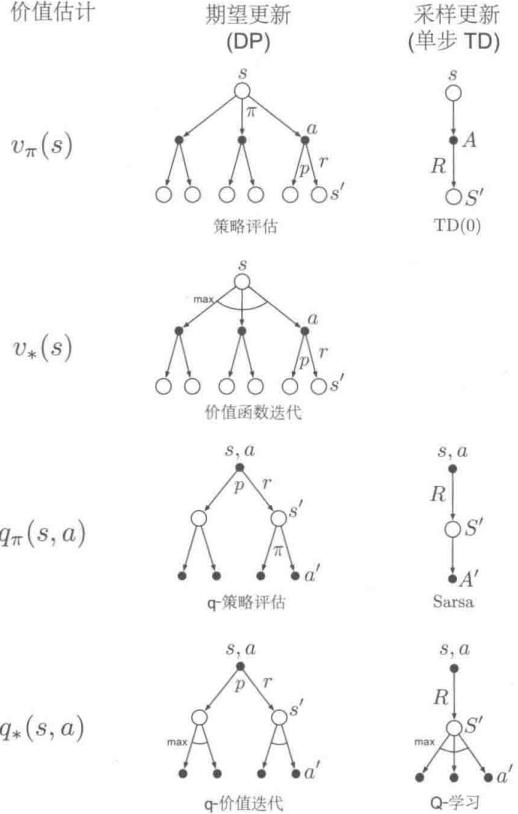
\includegraphics[width=0.6\textwidth]{compare_update}
\caption[表格型方法更新对比]{更新对比}
\end{figure}
%------------------------------------------------
\paragraph{规划}
\begin{itemize}
\item 后台规划:从环境模型生成模拟经验,改进策略或价值函数
\begin{itemize}
\item 表格型方法
\item 近似方法
\end{itemize}
\item 决策时规划:使用模拟经验为当前状态选择动作
\end{itemize}
%----------------------------------------------------------------------------------------
\section{值函数近似}
%------------------------------------------------
\subsection{函数近似}
%------------------------------------------------
\paragraph{曲线拟合}
用少量参数储存状态,阶数越高越近似,且具有一定的泛化能力。
%------------------------------------------------
\paragraph{目标函数}
参数$ \omega $最小化目标函数$ J(\omega) = E[(v_{\pi}(S) - \hat{v}(S, \omega))^2] $。
%------------------------------------------------
\paragraph{状态分布}
\begin{itemize}
\item 均匀分布(各状态同等重要):$ J(\omega) = \frac{1}{|S|}\sum_{s \in S}(v_{\pi}(s) - \hat{v}(s, \omega))^2 $。
\item 平稳分布(马氏过程长期行为):$ J(\omega) = \sum_{s \in S}d_{\pi}(s)(v_{\pi}(s) - \hat{v}(s, \omega))^2 $。
\end{itemize}
%------------------------------------------------
\paragraph{优化算法}
梯度下降:$ \omega_{k + 1} = \omega_k - \alpha_k \nabla_\omega J(\omega_k) $

其中,
\begin{align*}
\nabla_\omega J(\omega)
&= \nabla_\omega E[(v_\pi(S) - \hat{v}(S, \omega))^2] \\
&= E[\nabla_\omega (v_\pi(S) - \hat{v}(S, \omega))^2] \\
&= 2E[(v_\pi(S) - \hat{v}(S, \omega))(-\nabla_\omega \hat{v}(S, \omega))] \\
&= -2E[(v_\pi(S) - \hat{v}(S, \omega)) \nabla_\omega \hat{v}(S, \omega)]
\end{align*}

因此$ \omega_{k + 1} = \omega_k + \alpha (v_\pi(s_k) - \hat{v}(s_k, \omega_k)) \nabla_\omega \hat{v}(s_k, \omega_k) $。
%------------------------------------------------
\paragraph{近似$ v_\pi(s_t) $}
\begin{itemize}
\item 蒙特卡洛:$ g_t $。
\item 时序差分:$ r_{t + 1} + \gamma \hat{v}(s_{t + 1}, \omega_t) $。
\end{itemize}
%------------------------------------------------
\paragraph{选取$ \hat{v}(S, \omega) $}
\begin{itemize}
\item 线性函数:$ \hat{v}(S, \omega) = \phi(S)^\top \omega $,表格法可视为其特殊情况。
\item 神经网络:输入状态,网络参数为$ \omega $,输出$ \hat{v}(S, \omega) $。
\end{itemize}
%------------------------------------------------
\subsection{深度Q学习(Deep Q-Network,DQN)}\tip{DQN(算法)}
深度Q学习用神经网络作为非线性函数近似器,最小化损失函数(贝尔曼最优性误差):
$$
J(\omega) = E[(R + \gamma \max_{a'} \hat{q}(S', a', \omega^-) - \hat{q}(S, A, \omega))^2]
$$
其中$ \omega $为主网络参数,$ \omega^- $为目标网络参数。
%------------------------------------------------
\paragraph{主要技术}
\begin{itemize}
\item 两个网络:主网络$ \hat{q}(S, A, \omega) $和目标网络$ \hat{q}(S', a', \omega^-) $,后者参数阶段性从前者同步(软/硬更新)。
\item 经验回放:打乱样本相关性,提升训练稳定性。
\end{itemize}
%------------------------------------------------
\paragraph{深度Q学习(离线)算法}
\begin{itemize}
\item 初始化主网络参数$ \omega $、目标网络参数$ \omega^- $,经验回放缓冲区$ B = \{(s, a, r, s')\} $
\item 循环:
\begin{itemize}
\item 从$ B $中均匀采样小批量样本$ \{(s, a, r, s')\} $
\item 计算目标值:$ y = r + \gamma \max_{a'} \hat{q}(s', a', \omega^-) $
\item 用小批量样本$ \{(s, a, y)\} $更新主网络,最小化$ (y - \hat{q}(s, a, \omega))^2 $
\item 每隔$ C $步令$ \omega^- = \omega $
\end{itemize}
\end{itemize}
%----------------------------------------------------------------------------------------
\section{附录}
%------------------------------------------------
\subsection{历史}
\begin{enumerate}
\item 源于动物学习心理学的试错法:效应定律(Edward Thorndike),条件反射(巴普洛夫),快乐-痛苦系统(图灵),向“老师”学习到向“评论家”学习,自动学习机(M.L.Tsetlin),分类器系统(救火队算法和遗传算法)。
\item 最优控制:贝尔曼方程与马尔可夫决策过程(Richard Bellman),维度灾难。
\item 时序差分方法:次级强化物,广义强化(Klopf),与试错法结合(“行动器-评判器”结构,Sutton),与最优控制结合(Q-learning,Chris Watkins)。
\end{enumerate}
%------------------------------------------------
\subsection{贝尔曼最优方程求解}\label{sec:Scalability Mapping}
%------------------------------------------------
\paragraph{收缩映射定理}
若$ f(x) $是收缩映射,则存在唯一一个不动点$ x^* $满足$ f(x^*) = x^* $。针对$ x_{k + 1} = f(x_k) $,在$ x_k \to x^*, k \to \infty $的过程中,收敛速度成指数级增长。
\begin{itemize}
\item 存在性:$ ||x_{k + 1} - x_k|| = ||f(x_{k + 1}) - f(x_k)|| \leq \gamma||x_k - x_{k - 1}|| \leq \dots \leq \gamma^k||x_1 - x_0|| $,由于$ \gamma < 1 $,$ \gamma^k \to 0 $,所以$ x_{k + 1} - x_k \to 0 $。同理可得$ ||x_m - x_n|| \leq \frac{\gamma^n}{1 - \gamma}||x_1 - x_0|| \to 0 $。进而得到$ \{x_k\} $是收敛数列,存在$ \lim_{k \to \infty} x_k = x^* $。
\item 唯一性:$ ||f(x_k) - x_k|| = ||x_{k + 1} - x_k||$,其快速收敛到$ 0 $,则在极限处有不动点$ f(x^*) = x^* $。假设存在另一不动点,其必与该不动点相等。
\item 指数级收敛:$ ||x^* - x_n|| = \lim_{m \to \infty}||x_m - x_n|| \leq \frac{\gamma^n}{1 - \gamma}||x_1 - x_0|| \to 0 $。
\end{itemize}
%------------------------------------------------
\paragraph{贝尔曼最优方程的伸缩映射性}~\\

$ \forall v1,v2 $,有贝尔曼最优方程$ \pi_i^* \doteq \arg \max_{\pi} (r_\pi + \gamma P_\pi v_i) $,

故$ f(v_i) = \max_{\pi} (r_\pi + \gamma P_\pi v_i) = r_{\pi_i^*} + \gamma P_{\pi_i^*} v_i \geq r_{\pi_j^*} + \gamma P_{\pi_j^*} v_i (i \neq j) $,

则
\begin{align*}
f(v_1) - f(v_2) 
&= r_{\pi_1^*} + \gamma P_{\pi_1^*} v_1 - (r_{\pi_2^*} + \gamma P_{\pi_2^*} v_2) \\
&\leq r_{\pi_1^*} + \gamma P_{\pi_1^*} v_1 - (r_{\pi_1^*} + \gamma P_{\pi_1^*} v_2) \\
&= \gamma P_{\pi_1^*} (v_1 - v_2)
\end{align*}

同理有$ f(v_2) - f(v_1) \leq \gamma P_{\pi_2^*} (v_2 - v_1) $,

故$ \gamma P_{\pi_2^*} (v_1 - v_2)\leq f(v_1) - f(v_2) \leq \gamma P_{\pi_1^*} (v_1 - v_2) $,

取边界极值$ z $,有$ |f(v_1) - f(v_2)| \leq z $,即$ ||f(v_1) - f(v_2)||_\infty \leq ||z||_\infty $。

又有$ ||z||_\infty = max_i |z_i| \leq \gamma ||v_1 - v_2||_\infty $,所以$ ||f(v_1) - f(v_2)||_\infty \leq \gamma ||v_1 - v_2||_\infty $。

故贝尔曼最优方程有伸缩映射性。
%------------------------------------------------
\paragraph{贝尔曼最优方程解的性质}
\begin{itemize}
\item 唯一性:唯一解$ v^* $能通过$ v_{k + 1} = f(v_k) = \max_{\pi \in \Pi} (r_\pi + \gamma P_\pi v_k) $迭代求解,其对应策略$ \pi^* = argmax_{\pi \in \Pi} (r_\pi + \gamma P_\pi v^*) $。
\item 最优性($ v^* = v_{\pi^*} \geq v_{\pi} $):
由$ v_{\pi} = r_{\pi} + \gamma P_{\pi} v_{\pi} $和$ v^* = \max_{\pi} (r_{\pi} + \gamma P_{\pi} v^*) = r_{\pi^*} + \gamma P_{\pi^*} v^* \geq r_{\pi} + \gamma P_{\pi} v^* $,
可得$ v^* - v_{\pi} \geq (r_{\pi} + \gamma P_{\pi} v^*) - (r_{\pi} + \gamma P_{\pi} v_{\pi}) = \gamma P_{\pi} (v^* - v_{\pi}) $,
即有$ v^* - v_{\pi} \geq \gamma P_{\pi} (v^* - v_{\pi}) \geq \dots \geq \gamma^n P_{\pi}^n (v^* - v_{\pi}) $,
由于$ \gamma < 0 $,$ \forall p_{ij} \in P_{\pi}, p_{ij} \leq 1 $,$ \lim_{n \to \infty} \gamma^n P_{\pi}^n (v^* - v_{\pi}) $趋于0,所以$ v^* \geq v_{\pi} $。
\end{itemize}

返回正文\ref{sec:Scalability Mapping back}。
%------------------------------------------------
\subsection{数学基础}
%------------------------------------------------
\paragraph*{概率空间$ (\Omega, F, P) $}
\begin{itemize}
\item 性质
\begin{itemize}
\item 非负性:$ \forall A \in F,P(A) \geq 0 $。
\item 规范性:$ P(\Omega) = 1 $。
\item 可列可加性:若$ A_1, A_2, \dots $互斥,则$ P(\bigcup_{i = 1}^{\infty} A_i) = \sum_{i = 1}^{\infty} P(A_i) $。
\end{itemize}
\item 运算
\begin{itemize}
\item 补集:$ P(A^c) = 1 - P(A) $。
\item 交集:$ P(A \cap B) = P(A) + P(B) - P(A \cup B) $。
\end{itemize}
\end{itemize}
%------------------------------------------------
\paragraph*{随机变量}
\begin{itemize}
\item 离散型
\begin{itemize}
\item 概率质量函数(PMF):$ P(X = x) = p(x) $,满足 $ \sum_{x} p(x) = 1 $。
\item 期望:$ E[X] = \sum_{x} x p(x) $。
\item 方差:$ Var(X) = E[(X - E[X])^2] $。
\end{itemize}
\item 连续型
\begin{itemize}
\item 概率密度函数(PDF):$ f(x) \geq 0 $,满足$ \int_{-\infty}^{\infty} f(x) dx = 1 $。
\item 期望:$ E[X] = \int_{-\infty}^{\infty} x f(x) dx $。
\item 方差:$ Var(X) = E[(X - E[X])^2] $。
\end{itemize}
\end{itemize}
%------------------------------------------------
\paragraph*{条件概率与独立性}
\begin{itemize}
\item 条件概率:$ P(B|A) = \frac{P(A \cap B)}{P(A)}$当$ P(A) > 0 $。
\item 全概率公式:$ P(B) = \sum_{A \subseteq F} P(B|A) P(A) $。
\item 贝叶斯定理:$ P(A|B) = \frac{P(B|A) P(A)}{P(B)} $。
\item 独立性: $ A,B $独立$ \iff P(A \cap B) = P(A)P(B) $。
\item 条件独立:$ P(A ,B|C) = P(A|C)P(B|C) $。
\end{itemize}
%------------------------------------------------
\paragraph*{马尔可夫链与转移概率}
\begin{itemize}
\item 马尔可夫性:$ P(S_{t + 1}|S_t, S_{t - 1}, \dots, S_0) = P(S_{t + 1}|S_t) $。
\item 转移矩阵:$ P \in [0, 1]^{S \times S}, P(s'|s) = \sum_{a} P(s'|s, a) P(a|s) $。
\item 平稳分布:$ \pi = \pi P $,即$ \pi(s') = \sum_{s} \pi(s) P(s'|s) $。
\end{itemize}
%------------------------------------------------
\paragraph*{大数定律与中心极限定理}
\begin{itemize}
\item 弱大数律:$ \frac{1}{n} \sum_{i=1}^n X_i \overset{p}{\Longrightarrow} E[X] $。
\item 强大数律:$ \frac{1}{n} \sum_{i=1}^n X_i \overset{a.s.}{\Longrightarrow} E[X] $。
\item 中心极限定理:$ X_1, X_2, \dots $独立同分布,均值为$ \mu $,方差为$ \sigma^2 < \infty $,则$ \frac{1}{\sqrt{n}} \sum_{i=1}^n (X_i - \mu) \overset{d}{\Longrightarrow} N(0, \sigma^2) $。
\end{itemize}
%------------------------------------------------
\paragraph*{泛函分析}
\begin{itemize}
\item 期望的线性:$ E[aX + bY] = a E[X] + b E[Y] $。
\item 协方差:$ Cov(X, Y) = E[(X - \mu_X)(Y - \mu_Y)] = E[XY] - \mu_X \mu_Y $。
\item 相关系数:$ \rho(X, Y) = \frac{Cov(X, Y)}{\sigma_X \sigma_Y} $。
\end{itemize}
%----------------------------------------------------------------------------------------
\end{document}